%%%%%%%%%%%%%%%%%%%%%%%%%%%%%%%%%%%%%%%%%%%%%%%%%%%%%%%%%%%%%%%%%%
% Sample template for MIT Junior Lab Student Written Summaries
% Available from http://web.mit.edu/8.13/www/Samplepaper/sample-paper.tex
%
% Last Updated August 30, 2011
%
% Adapted from the American Physical Societies REVTeK-4.1 Pages
% at http://publish.aps.org
%
% ADVICE TO STUDENTS: Each time you write a paper, start with this
% template and save under a new filename. If convenient, don't
%    erase unneeded lines, just comment them out.  Often, they
%    will be useful containers for information.
%
% Using pdflatex, images must be either PNG, GIF, JPEG or PDF.
%     Turn eps to pdf using epstopdf.
%%%%%%%%%%%%%%%%%%%%%%%%%%%%%%%%%%%%%%%%%%%%%%%%%%%%%%%%%%%%%%%%%%


%%%%%%%%%%%%%%%%%%%%%%%%%%%%%%%%%%%%%%%%%%%%%%%%%%%%%%%%%%%%%%%%%%
% PREAMBLE
% The preamble of a LaTeX document is the set of commands that precede
% the \begin{document} line.  It contains a \documentclass line
% to load the REVTeK-4.1 macro definitions and various \usepackage
% lines to load other macro packages.
%
% ADVICE TO STUDENTS: This preamble contains a suggested set of
% class options to generate a ``Junior Lab'' look and feel that
% facilitate quick review and feedback from one's peers, TA's
% and section instructors. Don't make substantial changes without
%     first consulting your section instructor.
%%%%%%%%%%%%%%%%%%%%%%%%%%%%%%%%%%%%%%%%%%%%%%%%%%%%%%%%%%%%%%%%%%

\documentclass[aps,twocolumn,secnumarabic,balancelastpage,amsmath,amssymb,nofootinbib]{revtex4}
%\documentclass[aps,twocolumn,secnumarabic,balancelastpage,amsmath,amssymb,nofootinbib]{revtex4-1}
\pdfpagewidth 8.5in
\pdfpageheight 11in

\usepackage{lgrind} % convert program listings to a form includable in a LaTeX document
\usepackage{chapterbib} % allows a bibliography for each chapter(each labguide has it's own)
\usepackage{color} % produces boxes or entire pages with coloredbackgrounds
\usepackage{graphics}      % standard graphics specifications
\usepackage[pdftex]{graphicx} % alternative graphics specifications
\usepackage{longtable}     % helps with long table options
\usepackage{epsf} % old package handles encapsulated post scriptissues
\usepackage{bm}            % special 'bold-math' package
%\usepackage{asymptote} % For typesetting of mathematical illustrations
\usepackage{thumbpdf}
\usepackage[colorlinks=true]{hyperref} % this package should be added after all others
% use as follows: \url{http://web.mit.edu/8.13}
\usepackage{multirow}
\usepackage{subfigure}

% Define a useful new command for writing units
\newcommand{\cd}{$\cdot$}

%
% And now, begin the document...
%

\begin{document}
\title{M{\"o}ssbauer Spectroscopy in $^{57}Fe$ Compounds}
\author{Jay M.\ Lawhorn}
\email{klawhorn@mit.edu}
\date{\today}
\affiliation{MIT Department of Physics}

\begin{abstract}
M{\"o}ssbauer spectroscopy with a $^{57}_{27}$Co source is used to probe atomic energy level effects in iron compounds, including Zeeman splitting and electric quadrupole effects. The ratio of magnetic moments in the first excited state and ground state in metallic iron is measured to be $-1.709\pm0.066$, which is consistent with the literature value. A similar value is measured in Fe$_2$O$_3$, but no significant isomer or electric quadrupole shift is observed for that compound. The natural line width of the 14.4 keV transition at room temperature is measured to be $(1.46\pm0.48)\times 10^{-8}$ eV, $2.5\sigma$ above the literature value.
\end{abstract}

\maketitle

When an atom of $^{57}$Fe in the first excited state transitions to the ground state, it emits a 14.4 keV gamma ray. As described in Reference \cite{lab}, this specific transition has an extremely small natural line width of $4.7\times10^{-9}$ eV, making it an excellent candidate for precision spectroscopy with a potential resolution of $E/\Delta E \approx 10^{12}$. 

However, the atomic transition conserves momentum so the emitting atom recoils and resulting gamma ray energy is slightly lower that 14.4 keV. Similarly, a slightly higher energy gamma ray is needed to excite the same transition. The net result is that a 14.4 keV gamma ray emitted by a free $^{57}$Fe atom is unlikely to be absorbed by another$^{57}$Fe atom.

Rudolph M{\"o}ssbauer developed a method to increase the the probability of nuclear resonance fluorescence by embedding the atom of interest in a lattice and was awarded the 1961 Nobel prize for his observation of the phenomenon in $^{191}$Ir. When an atom in a lattice structure emits a gamma ray, the entire lattice structure will recoil together, greatly increasing the effective mass and minimizing the energy loss. This is known as recoilless emission. 

Embedded in the right lattice structure, $^{57}$Fe is an excellent choice because an estimated 90\% \cite{mel} of emitted gamma rays will be emitted without recoil. In this experiment a specially prepared M{\"o}ssbauer source consisting of $^{57}_{27}$Co diffused in a platinum substrate is used. The $^{57}_{27}$Co decays by K-electron capture to the second excited state of $^{57}$Fe. 91\% of atoms in the second excited state subsequently transition to the first excited state, which then transitions to the ground state via emission of a 14.4 keV gamma ray. These gamma rays are much more likely to excite the same transition in another $^{57}$Fe atom than in the free atom case. Such an event is an example of nuclear resonance fluorescence. 

This ultra-narrow emission line is used to probe nearby energies by introducing a relative velocity $V$ which creates an energy shift given by 
\begin{equation}
E' = E \left(1+\frac{V}{c} \right)
\label{eq:dop}
\end{equation}
where $E$ is 14.4 keV and $c$ is the speed of light.

\begin{figure}[htb]
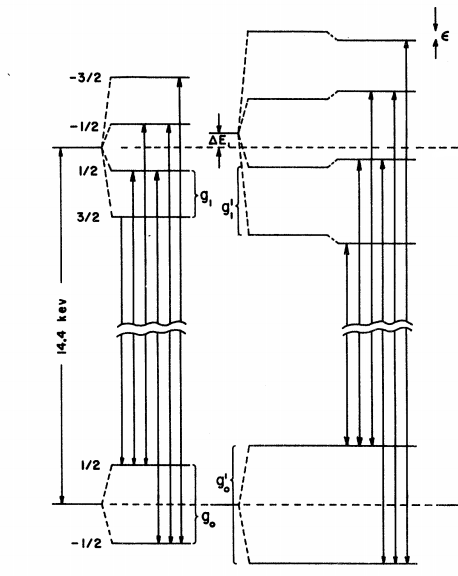
\includegraphics[width=6cm]{spec.png}
\caption{(left) Zeeman splittings in the first two levels of metallic iron. Note that the first excited state splitting is inverted with respect to the ground state. (right) Zeeman and electric quadrupole splittings in the first two levels of iron in $Fe_2O_3$. Reproduced from Reference \cite{kistner}.}
\label{fig:spec}
\end{figure}

M{\"o}ssbauer spectroscopy is used to probe atomic energy splittings and shifts, as illustrated in Figure \ref{fig:spec}. 

At left are the energy splittings and allowed transitions in metallic iron, which has an internal magnetic field that induces a hyperfine Zeeman splitting. Of the eight possible transitions between the spin-1/2 ground state and spin-3/2 excited state, two are forbidden to first order by magnetic-dipole selection rules. The ratio of magnetic moments in the first excited state and the ground state is 
\begin{equation}
\frac{\mu_1}{\mu_0} = \frac{-3\Delta E_1}{\Delta E_0}
\label{eq:mag}
\end{equation}
where $\Delta E_1$ is the energy difference between two adjacent energy levels in the excited state and $\Delta E_0$ is the energy difference between the two energy levels of the ground state.

The magnetic moment of the first excited state is determined from this ratio and the measurement described in Reference \cite{ludwig} of the magnetic moment of the ground state of iron as $\mu_0=0.0903\pm0.0007$ nm. 

At right are the transitions in $Fe_2O_3$, which exhibits an electric quadrupole moment as well as a magnetic moment. The electric quadrupole moment introduces an energy shift of magnitude $\epsilon$ in the energy levels of the excited state which is positive in the two middle states and negative in the remaining two states.

The diagram also depicts an isomer shift between the two spectra parameterized by $\Delta E_L$. The isomer shift is the result of different chemical environments in the source and absorber resulting in an overall shift in the center of gravity of the six absorption lines. 

The experimental setup is shown in Figure \ref{fig:setup} and exact equipment models are given in Reference \cite{lab}. The $^{57}_{27}$Co source is mounted on an oscillating piston controlled by a programmable M{\"o}ssbauer drive. A proportional gas counter is used to detect gamma rays emitted by the source through a solid absorber containing iron. The signal from the counter is amplified and sent through a multi-channel scaler. A discriminator threshold for the scaler is set to exclude the 6.4 keV gamma rays emitted in the electron capture decay of $^{57}_{27}$Co. The scaler records detected photons in 100$\mu$s time intervals. 

\begin{figure}[htb]
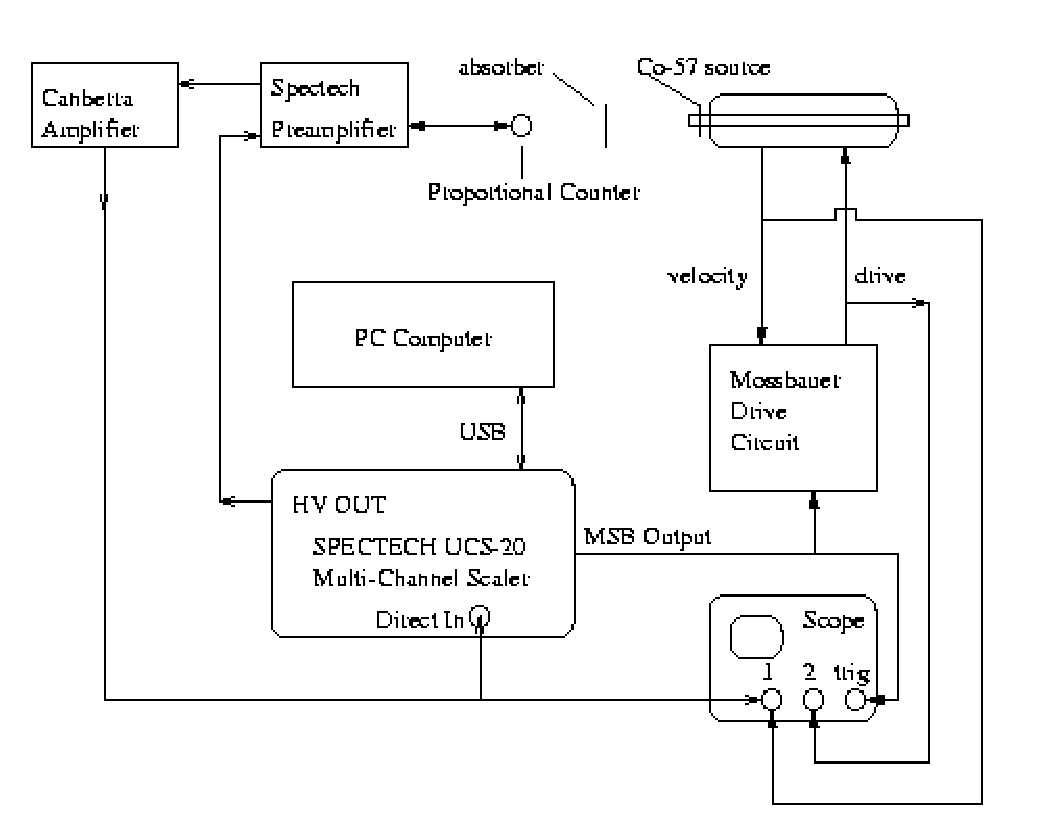
\includegraphics[width=8cm]{setup.png}
\caption{Experimental setup. The source is mounted on a piston controlled by a M{\"o}ssbauer drive and a proportional counter detects emitted gamma rays after transmission through the selected absorber. A multi-channel scaler integrates data over a given time interval, which is read out and processed via computer. }
\label{fig:setup}
\end{figure} 

The piston is set to oscillate with a periodic sawtooth function of velocity at 5 Hz. The scaler is set to bin the acquired photon counts in 2048 consecutive time intervals at 5 Hz such that each bin corresponds to a specific relative velocity of source and absorber. Absorption lines corresponding to specific transition energies in the absorber are observed as Lorentzian deficits in the count rate with relative velocity on a continuum spectra consisting of the non-recoilless component of the 14.4 keV source emission line. 

The absolute velocity of the piston is measured using an adjacent interferometer. Light from a 623.8 nm laser is split, reflected off either a mirror attached to the piston or a fixed mirror, and recombined into a photodiode. The photodiode signal is amplified and processed such that each interference peak corresponding to a change in piston position of one wavelength generates a digital logic 1 pulse. This signal is passed to the same multi-channel scaler described above, and the change in distance in units of the laser wavelength is recorded for each of the 2048 time intervals across the piston oscillation.

The change in distance per time interval is converted to a velocity $V_i$ for that bin by
\begin{equation}
V_i = \frac{C\lambda}{2NT}
\label{eq:v}
\end{equation}
where $C$ is the number of counts in that bin, $\lambda$ is the wavelength of light, $N$ is the number of passes, and $T$ is the dwell time per channel such that $NT$ is the total data acquisition time per channel.

The velocity at each bin is calculated using Equation \ref{eq:v} and data acquired over a total dwell time of 0.23 sec per bin from 2,323 piston oscillations with a dwell time of 100 $\mu$s per bin per oscillation. The resulting curve is shown in Figure \ref{fig:inter}. The first hundred bins correspond to a very rapid reset period that is excluded from further analysis. The rest of the bins correspond to sawtooth function of velocity, with zero relative velocity at approximately bin 1000 and large bins corresponding to the piston moving towards the source. 

\begin{figure}[htb]
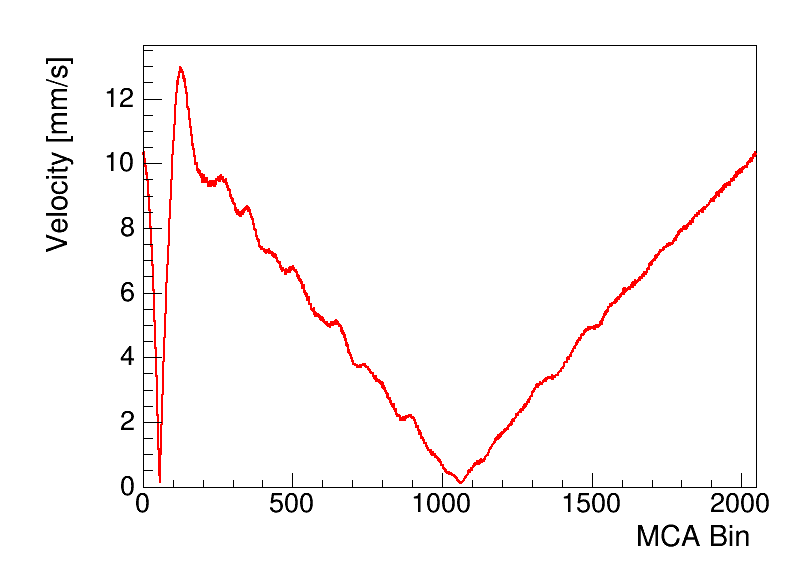
\includegraphics[width=8cm]{inter_paper.png}
\caption{Velocity at 2048 time intervals across the period of a piston oscillation. The oscillatory behavior observed is a result of background contamination that produces intensity peak in the photodiode.}
\label{fig:inter}
\end{figure}

Two strategies are explored for the fit to the interferometric velocity data. The first is a fit of the form $a_0+|a_1(x-a_2)+a_3(x-a_2)^2|$ over the entire velocity spectrum, and the second is fitting two separate linear functions to regions on either side of the cusp and patching them together at their intersection. The average value of $(y_{\mathrm{fit}}-y_{\mathrm{data}})/y_{\mathrm{fit}}$ for each strategy is computed. The first fit strategy is selected based on a calculated value of $1.2\times10^{-4}$ compared to $6.6\times10^{-3}$ for the second strategy. 

In both strategies, the largest discrepancy is near the cusp, which is most sensitive to background effects and the observed ringing phenomenon. The difference in resulting velocity at a specific bin from the two fit strategies is taken as the uncertainty in the velocity determination instead of the discrepancy between fit and data because the latter is much more sensitive to the ringing phenomenon instead of the overall trend in the underlying process.

An uncertainty is also evaluated for the choice of lower cutoff for the fit range in the single-fit strategy. The nominal value for this cutoff is chosen as bin 200. Fits to the data with even lower cutoffs were found to differ more from the data using the same figure of merit as described above, but the uncertainty stemming from this choice is evaluated as the difference in calculated velocity using a fit to data above bin 200 and using a fit to data above bin 100. 

The observed spectrum through a metallic $^{57}$Fe absorber over 0.65 seconds per bin is shown in Figure \ref{fig:metal}. Each absorption line is assumed to be a Lorentzian of the form
\begin{equation}
I = \frac{I_0 (\Gamma/2)^{2}}{(E - E_0)^{2}+(\Gamma/2)^2}
\label{eq:lor}
\end{equation}
where $I_0$ describes the peak height, $E_0$ is the center energy, and $\Gamma$ is the full-width at half-maximum. The non-recoilless emission background that comprises the continuum spectrum is assumed to be quadratic. The spectrum is fit to the sum of six Lorentzians and a quadratic background.

\begin{figure}[htb]
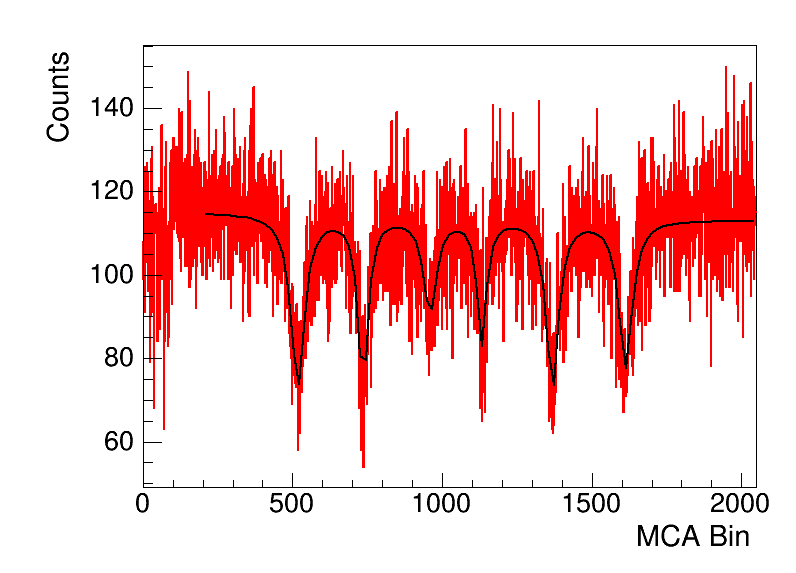
\includegraphics[width=8cm]{fePeaks.png}
\caption{Observed spectrum for a metallic iron absorber.}
\label{fig:metal}
\end{figure}

The $E_0$ parameter for each peak is taken to be the bin number of the line center, with the uncertainty in line location estimated by $\sqrt{\Gamma}$. The bin number is translated to a velocity using the nominal fit to the interferometric data. The uncertainty in velocity calibration is assessed as described above, and the uncertainty in line center is propagated through the nominal velocity formula. The measured velocities of the six absorption lines are listed in Table \ref{table:vel}. 

\begin{table}[h]
\caption{\label{table:vel} Velocities of the six metallic iron peaks. The uncertainties from line center determination, choice of the fit range, and choice of the velocity functional form are listed in that order. }
\begin{tabular}{|c|}
\hline
Velocity [mm/s] \\
\hline
$-6.16 \pm 0.12 \pm 0.07 \pm 0.09$ \\
\hline
$-3.63 \pm 0.14 \pm 0.03 \pm 0.07$ \\
\hline
$-1.10 \pm 0.08 \pm 0.00 \pm 0.08$ \\
\hline
$0.82 \pm 0.05 \pm 0.01 \pm 0.07$ \\
\hline
$3.37 \pm 0.02 \pm 0.02 \pm 0.08$ \\
\hline
$5.92 \pm 0.08 \pm 0.01 \pm 0.08$ \\
\hline
\end{tabular}
\end{table}

The various energy splittings are computed as the difference between various line centers with reference to Figure \ref{fig:spec}. For parameters that can be calculated from multiple pairs of absorption lines, all possible differences are computed and the weighted average is reported. The calculated parameters are tabulated in Table \ref{tab:end}.

All uncertainties are assumed to be completely uncorrelated and are added in quadrature. The uncertainty in line center from the line width and choice of functional form for the velocity curve are equally important effects, while the choice of fit range is most significant in the lower bins near the lower threshold. 

From the Zeeman energy splittings and Equation \ref{eq:mag} the ratio of magnetic moments in the first excited state and ground state is computed to be $-1.709\pm0.066$. This is consistent with the value $-1.715\pm0.004$ given in Reference \cite{preston}. Using the known value of the ground state magnetic moment, the magnetic moment of the first excited state is computed to be $-0.1543 \pm0.0061$ nm.

The observed spectrum through a $Fe_2O_3$ absorber over 2.5 minutes per bin is shown in Figure \ref{fig:fe2o3}. The same line center extraction method and uncertainty estimation as in metallic iron is used. 
 
\begin{figure}[htb]
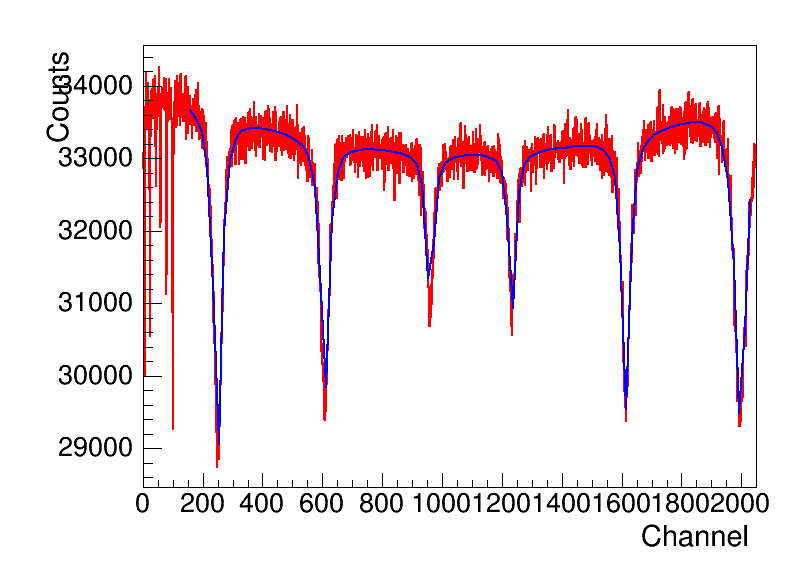
\includegraphics[width=8cm]{fe2o3_peaks.png}
\caption{Observed spectrum for a $Fe_2O_3$ absorber.}
\label{fig:fe2o3}
\end{figure}

The velocity calibration for this sample is made using a metallic iron spectrum taken immediately beforehand with the same settings. The measured velocities from the interferometric calibration are plotted against the six metallic iron lines centers and associated uncertainties extracted from the secondary calibration spectrum. A quadratic polynomial is fit to the six points. 

The difference in velocity between the interferometric velocity and the output of the fitted polynomial at the measured bin center is computed for each line center. The difference between the interferometric velocity and the polynomial fit is observed to increase as distance from the nominal zero velocity point increases. The uncertainty in velocity determination for each of the observed lines in $Fe_2O_3$ is estimated by fitting a quadratic polynomial to the difference in calculated velocities as a function of bin number. 

Evaluating the uncertainties in this way reflects both the differences between the interferometry-derived values and the secondary calibration and the fact that the two extreme absorption lines in $Fe_2O_3$ fall outside the metallic iron lines and should therefore have substantial uncertainty because of potential non-linearities in the regions not represented in the fits. 

The various energy splittings are computed as the difference between various line centers with reference to Figure \ref{fig:spec}.  All uncertainties are assumed to be completely uncorrelated and are added in quadrature. For parameters that can be calculated from multiple pairs of absorption lines, all possible differences are computed and the weighted average is reported. The calculated parameters are tabulated in Table \ref{tab:end}.

For this measurement, the uncertainty in velocity calibration dominates across this spectrum. The extended integration time minimized the line width uncertainty compared to the much shorter integration time for metallic iron. The precision of this measurement could be improved by using an interferometric velocity calibration. 

In $Fe_2O_3$, the ratio of magnetic moments for the first excited state and ground state is found to be $-1.718\pm0.068$, which is consistent with both the metallic iron measurement and the literature value given above. The measured electric quadrupole moment shift and isomer shift in $Fe_2 O_3$ are consistent with zero. The electric quadrupole moment is known to be non-zero, but its measurement is especially sensitive to experimental uncertainties because its calculation involves four different line locations instead of the two that the energy splittings require. It is likely that a dramatic improvement in precision is needed to make a measurement of this parameter. 

A series of six ferrocyanide absorbers of varying thickness ranging from 25 mg/cm$^{2}$ to 150 mg/cm$^{2}$ are used to evaluate the natural line width of the 14.4 keV transition. Ferrocyanide has no magnetic field at the iron nucleus and thus there is only one observed absorption peak corresponding to no energy level splitting. For each source, approximately 45 seconds of data per bin are acquired. 

A single Lorentzian absorption peak on a constant background is fit to the acquired data on a restricted range corresponding to the central 300 MCA bins to reduce the impact of background structure resulting from impurities in the absorber on the fit. The full-width half-maximum $\Gamma$ for each fit describes the line width at each thickness. The reported uncertainty in this parameter from the fit is taken as an uncertainty on the line width determination. A representative spectrum acquired with the 50 mg/cm$^{2}$ ferrocyanide absorber is shown in Figure \ref{fig:cn}. 

\begin{figure}[htb]
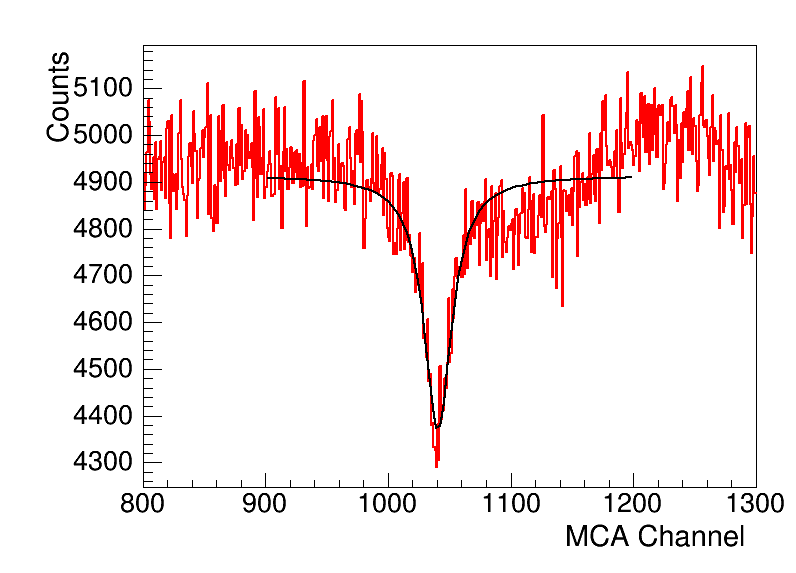
\includegraphics[width=8cm]{linewidth22.png}
\caption{Observed spectrum for the 50 mg/cm$^{2}$ ferrocyanide absorber. The apparent structure immediately to the right of the absorption line is observed in three of the six spectra. }
\label{fig:cn}
\end{figure}

The uncertainty in each line width measurement from the non-linearity of the velocity calibration is conservatively estimated as the uncertainty in velocity at the center of the peak. The cusp region had the largest deviation between the observed data and the intersection of two straight lines in the interferometric measurements as well as the largest deviation between the two interferometric fit strategies which indicates the potential for significant non-linearities in this region. 

\begin{figure}[htb]
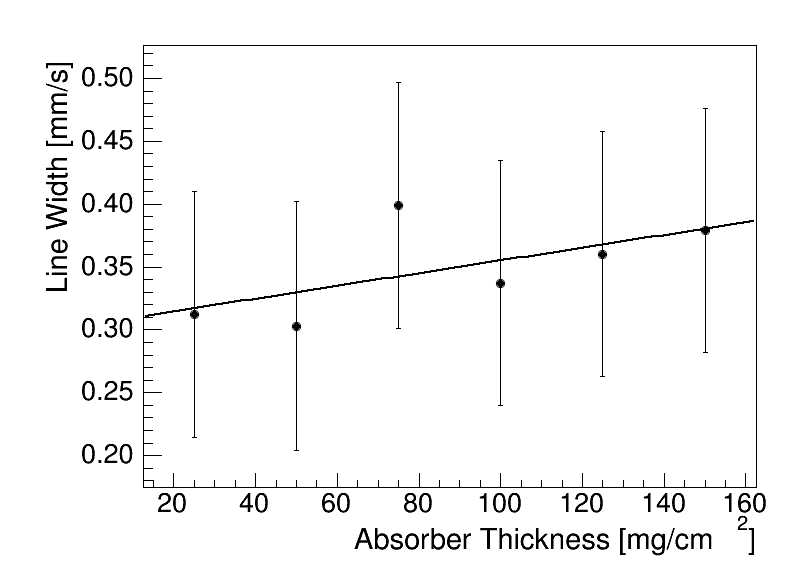
\includegraphics[width=8cm]{linewidth.png}
\caption{Calculated line width in mm/s of the 14.4 keV absorption line in ferrocyanide as a function of absorber thickness.}
\label{fig:width}
\end{figure}

A straight line is fit to the six data points, and the constant term is interpreted as the natural line width of the 14.4 keV line for an absorber of zero thickness. It is calculated as $(1.46\pm0.48)\times 10^{-8}$ eV, which is inconsistent with $4.7\times10^{-9}$ eV, the given line width in Reference \cite{lab}, at 2.5$\sigma$. This is likely due to thermal motion at the single atom level that is not related to line saturation effects and thus not removed by extrapolation to a zero-thickness absorber. 

The potential bias in limiting the fit region is evaluated by extending the fit region to the central 500 MCA bins, which includes the structure to the right of the absorption line in Figure \ref{fig:cn}. The zero-thickness line width in this case is calculated to be $(1.65\pm0.49)\times 10^{-8}$ eV, indicating that there is a noticeable effect on the expected natural line width, but it is smaller than the measurement uncertainty. A better understanding of this structure and its origins will improve the natural line width measurement, though measurements at room temperature are not expected to achieve the literature value for the natural line width. 

A summary of all numerical results is given in Table \ref{tab:end}. The energy level splits in metallic iron and $Fe_2O_3$ and the derived ratio of magnetic moments of the lowest two states of iron are consistent with the literature values. The isomer shift in both materials and the electric quadrupole moment of $Fe_2O_3$ are found to be consistent with zero, in contradiction to the literature. The predicted isomer and electric quadrupole shifts are much smaller than the Zeeman splittings, and increased precision would likely yield significant measurements of these effects. The natural line width of the 14.4 keV transition is measured to be much larger than the literature value for this parameter. 

\begin{table}[h]
\caption{\label{tab:end} Summary of results.}
\begin{tabular}{|c|c|c|}
\hline
Parameter & System & Value \\
\hline
$\Delta E_0$ & $^{57}$Fe & $(2.126\pm0.052)\times 10^{-7}$ eV \\
\hline
$\Delta E_1$ & $^{57}$Fe & $(1.211\pm0.036)\times 10^{-7}$ eV \\
\hline
$\mu_1 / \mu_0$ & $^{57}$Fe & $-1.709\pm0.066$ \\
\hline
$\Delta E_{\mathrm{Iso}} $ & $^{57}$Fe & $(-6.1\pm14.4)\times 10^{-9}$ eV \\
\hline
$\Delta E_0$ & $Fe_2 O_3$ & $(3.347\pm0.066)\times 10^{-7}$ eV\\
\hline
$\Delta E_1$ & $Fe_2 O_3$ & $(1.912\pm0.066)\times 10^{-7}$ eV \\
\hline
$\mu_1 / \mu_0$ & $Fe_2 O_3$ & $-1.718\pm0.068$ \\
\hline
$\epsilon$ & $Fe_2 O_3$ & $(6.3\pm10.4)\times 10^{-9}$ eV\\
\hline 
$\Delta E_{\mathrm{Iso}} $ & $Fe_2 O_3$ & $(1.5 \pm 2.0)\times 10^{-8}$ eV \\
\hline
$\Gamma $ & $Na_3Fe(CN)_6$ & $(1.46\pm0.48)\times 10^{-8}$ eV \\
\hline
\end{tabular}
\end{table}

The available precision of the apparatus could be greatly improved by using an interferometric velocity calibration for all measurements, but the required time to do so is prohibitive. This would allow for much greater velocity resolution because the six peaks of the metallic iron spectrum would not have to fall within the velocity range probed. It would be particularly useful for the natural line width determination because the absorption lines are much smaller than the metallic iron energy splitting.

\begin{thebibliography}{3}

\bibitem{lab}
8.14 staff, \emph{M{\"o}ssbauer Spectroscopy} Lab Guide, November 2012. 

\bibitem{mel}
A.C. Melissinos, \emph{M{\"o}ssbauer Effect} in Experiments in Modern Physics, Academic Press (New York 1966). 

\bibitem{ludwig}
G.W. Ludwig, H.H. Woodbury, \emph{Magnetic Moment of Fe$^{57}$}, Phys. Rev. 117, 1286 (1960).

\bibitem{preston}
R.S. Preston, S.S. Hanna, J. Heberle, \emph{M{\"o}ssbauer Effect in Metallic Iron}, Phys. Rev. 128, 2207 (1962). 

\bibitem{kistner}
O.C. Kistner, A.W. Sunyar, \emph{Evidence for Quadrupole Interaction of Fe$^{57m}$, and Influence of Chemical Binding on Nuclear Gamma-Ray Energy}, Phys. Rev. Lett. 4, 412 (1960).

\end{thebibliography}

\end{document}
